% Options for packages loaded elsewhere
\PassOptionsToPackage{unicode,}{hyperref}
\PassOptionsToPackage{hyphens}{url}
%
\documentclass[
  ]{scrartcl}
\usepackage{amsmath,amssymb}
\usepackage{iftex}
\ifPDFTeX
  \usepackage[T1]{fontenc}
  \usepackage[utf8]{inputenc}
  \usepackage{textcomp} % provide euro and other symbols
\else % if luatex or xetex
  \usepackage{unicode-math} % this also loads fontspec
  \defaultfontfeatures{Scale=MatchLowercase}
  \defaultfontfeatures[\rmfamily]{Ligatures=TeX,Scale=1}
\fi
\usepackage{lmodern}
\ifPDFTeX\else
  % xetex/luatex font selection
\fi
% Use upquote if available, for straight quotes in verbatim environments
\IfFileExists{upquote.sty}{\usepackage{upquote}}{}
\IfFileExists{microtype.sty}{% use microtype if available
  \usepackage[]{microtype}
  \UseMicrotypeSet[protrusion]{basicmath} % disable protrusion for tt fonts
}{}
\makeatletter
\@ifundefined{KOMAClassName}{% if non-KOMA class
  \IfFileExists{parskip.sty}{%
    \usepackage{parskip}
  }{% else
    \setlength{\parindent}{0pt}
    \setlength{\parskip}{6pt plus 2pt minus 1pt}}
}{% if KOMA class
  \KOMAoptions{parskip=half}}
\makeatother
\usepackage{xcolor}
\usepackage{graphicx}
\makeatletter
\def\maxwidth{\ifdim\Gin@nat@width>\linewidth\linewidth\else\Gin@nat@width\fi}
\def\maxheight{\ifdim\Gin@nat@height>\textheight\textheight\else\Gin@nat@height\fi}
\makeatother
% Scale images if necessary, so that they will not overflow the page
% margins by default, and it is still possible to overwrite the defaults
% using explicit options in \includegraphics[width, height, ...]{}
\setkeys{Gin}{width=\maxwidth,height=\maxheight,keepaspectratio}
% Set default figure placement to htbp
\makeatletter
\def\fps@figure{htbp}
\makeatother
\setlength{\emergencystretch}{3em} % prevent overfull lines
\providecommand{\tightlist}{%
  \setlength{\itemsep}{0pt}\setlength{\parskip}{0pt}}
\setcounter{secnumdepth}{-\maxdimen} % remove section numbering
\ifLuaTeX
\usepackage[bidi=basic]{babel}
\else
\usepackage[bidi=default]{babel}
\fi
\babelprovide[main,import]{american}
% get rid of language-specific shorthands (see #6817):
\let\LanguageShortHands\languageshorthands
\def\languageshorthands#1{}
\raggedbottom % or \flushbottom
% keep figures where there are in the text
\usepackage{float} 
\floatplacement{figure}{H}
% add custom hyphentation rules
\hyphenation
{%
  Hyphenate-me-like-this
  Dontyoueverhyphenateme
}%
\ifLuaTeX
  \usepackage{selnolig}  % disable illegal ligatures
\fi
\usepackage{bookmark}
\IfFileExists{xurl.sty}{\usepackage{xurl}}{} % add URL line breaks if available
\urlstyle{same}
\hypersetup{
  pdftitle={AUDIOSR - VAE},
  pdfauthor={Niv Aharon Cohen; Michael Berger},
  pdflang={en-US},
  hidelinks,
  pdfcreator={LaTeX via pandoc}}

\title{AUDIOSR - VAE}
\usepackage{etoolbox}
\makeatletter
\providecommand{\subtitle}[1]{% add subtitle to \maketitle
  \apptocmd{\@title}{\par {\large #1 \par}}{}{}
}
\makeatother
\subtitle{Subtitle}
\author{\href{mailto:nivcohen1000@gmail.com}{Niv Aharon
Cohen} \and \href{mailto:michael.berger.e@gmail.com}{Michael Berger}}
\date{17 September 2024}

\begin{document}
\maketitle
\begin{abstract}
In this project, we explored audio super-resolution by recreating and
enhancing the model proposed in AUDIOSR: Versatile Audio
Super-Resolution at Scale. Audio super-resolution aims to reconstruct
high-resolution audio from lower-resolution inputs, with applications in
areas such as music restoration, audio compression, and
telecommunication. The AUDIOSR model employs a diffusion-based
generative approach to upscale audio bandwidth from 2 kHz to 16 kHz,
generating high-resolution audio output at 24 kHz bandwidth with a 48
kHz sampling rate. Our work involved replicating the AUDIOSR
architecture and training process, while introducing some modifications
to further improve performance and versatility. We extended the model by
integrating additional features to filter different noises and
distortions. The performance of both the original and modified models
was evaluated on standard datasets, demonstrating competitive results in
terms of audio quality and bandwidth restoration. Our findings provide
insights into the adaptability of diffusion models in audio
super-resolution and open avenues for further research in this domain.
Our code demo is avaliable on Github on this link: PUT
LINK????????????????????????????
\end{abstract}



\renewcommand*\contentsname{Contents}
{
\setcounter{tocdepth}{1}
\tableofcontents
}
\listoffigures
\section{1. Introduction}\label{introduction}

Audio super-resolution (ASR) is the task of converting low-resolution
audio signals to high-resolution, enhancing their fidelity, bandwidth,
and perceptual quality. This problem is crucial in various fields,
including music production, audio restoration, and telecommunication,
where audio data often suffers from bandwidth limitations. As deep
learning techniques advance, several generative models have emerged,
offering new possibilities for tackling ASR with greater accuracy and
scalability.

One such model is AUDIOSR: Versatile Audio Super-Resolution at
Scale{[}????{]}, which leverages a diffusion-based generative framework
to reconstruct high-resolution audio from low-resolution inputs. The
model upscales audio bandwidth from 2 kHz to 16 kHz and generates
high-fidelity output with a bandwidth of 24 kHz and a sampling rate of
48 kHz. This approach marks a significant step forward in the domain of
ASR by effectively capturing the complex temporal and spectral
characteristics of audio signals. The AUDIOSR model builds upon earlier
work by Haohe Liu, particularly the AudioLDM{[}???????{]} framework.
AudioLDM was initially designed to convert text to audio by conditioning
audio generation on text during the training process. It introduces a
novel combination of Variational Autoencoders (VAE), Contrastive
Language-Audio Pretraining (CLAP), latent diffusion models, and audio
vocoders to synthesize high-quality audio. While AudioLDM focuses on
text-conditioned audio generation, AUDIOSR extends these ideas
specifically to bandwidth extension and high-resolution audio
reconstruction, focusing on the audio domain, but now with
audio-conditioning instead of text-conditioning. In this project, we
aimed to recreate the AUDIOSR model and extend its capabilities. Our
work introduces several modifications to improve the versatility and
performance of the model, including adjustments to the training process,
to train on different distortions and noises. This paper presents the
details of our implementation, the enhancements we introduced, and a
comprehensive evaluation of the model's performance.

\section{2. Literature Review}\label{literature-review}

One notable approach in the field of audio enhancement is presented by
Mostafa Sadeghi in ``Audio-visual Speech Enhancement Using Conditional
Variational Auto-Encoders'' {[}????{]} This study introduces a novel
method leveraging Conditional Variational Auto-Encoders (CVAEs) for
improving audio quality through the integration of visual information.
The method employs a dual VAE architecture, with one VAE dedicated to
processing audio and another to analyzing the visual representation of
the speaker's lips.

The core innovation of this approach lies in the conditioning of the
audio VAE on the visual VAE. By using lip movement data as a conditional
input, the model enhances the audio signal more effectively on the
additional contextual information provided by the visual data. This
approach mirrors the concepts explored in our project on audio super
resolution (AudioSR), where high-resolution audio is learned
conditionally based on low-resolution audio, with both signals encoded
using VAEs. The integration of visual data for audio enhancement
highlights the potential of using multi-modal information to improve
audio quality.

Another significant contribution to the field is presented by Huajian
Fang in ``Variational Autoencoder for Speech Enhancement with a
Noise-Aware Encoder'' {[}??????{]}. This study addresses the challenge
of noise reduction in speech enhancement through a sophisticated
VAE-based approach. Fang's method involves training two distinct VAEs:
one for clean audio and another for noisy audio. The purpose of this
dual VAE system is to encode both clean and noisy audio into separate
latent spaces.

A key aspect of this approach is the use of Kullback-Leibler (KL)
divergence to align the latent representations of noisy audio with those
of clean audio. By minimizing the divergence between these latent
spaces, the model effectively reduces the influence of noise, resulting
in enhanced speech quality. This noise-aware encoding technique
demonstrates a robust method for improving audio clarity by refining the
latent space representations. The concept of aligning noisy and clean
latent spaces shares similarities with our exploration of conditional
learning in AudioSR, underscoring the relevance of advanced VAE
techniques for effective audio enhancement.

\section{3. Problem Formulation And
Method}\label{problem-formulation-and-method}

Given an analog signal that has been discretely sampled at a rate of l
samples per second, resulting in a low-resolution sequence of values.
The goal of audio super resolution (SR) is to estimate a higher
resolution signal sampled at a rate of h samples per second, where h
\textgreater{} l. According to Nyquist's theory, the low resolution
signal have maximum frequency bandwidths of l/2 Hz and the high
resolution signal have h/2 Hz. Therefore, the information contained
between frequencies of h/2 − l/2 Hz is missing from the low resolution
signal. Estimating the ``missing'' frequency data is the core objective
of the SR task.

As outlined in the introduction, the entire AUDIOSR model builds upon
the author's previous work, AUDIOLDM. The architecture of AUDIOLDM
consists of several key components. First, the high-resolution audio is
converted into a Mel spectrogram, which is then encoded using a
Variational Autoencoder (VAE) to generate a latent space representation.
Simultaneously, the audio is encoded using the CLAP model to produce a
one-dimensional vector. Additionally, any conditional text is also
encoded using CLAP to create its own one-dimensional vector
representation.

Each encoded component---both the audio and the conditional text---is
then passed through the latent diffusion model, where sampling occurs.
Importantly, each part of the architecture is trained separately in a
sequential manner. Once processed, the data is passed through the VAE
decoder to reconstruct the Mel spectrogram. Finally, this spectrogram is
fed into a neural vocoder, which converts the Mel spectrogram back into
an audible audio signal.

\begin{figure}
\centering
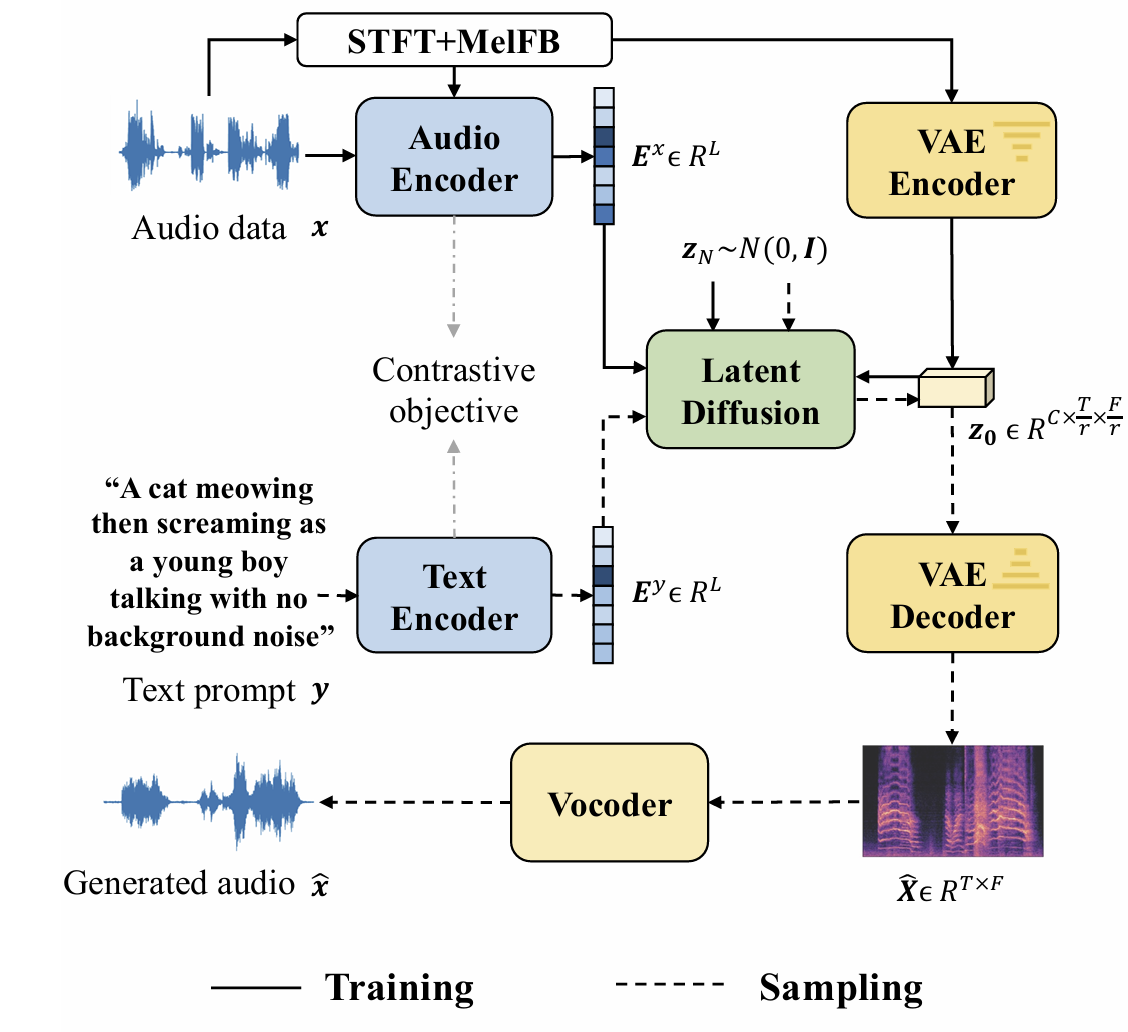
\includegraphics{images/audioldm_architecture_original.png}
\caption{Architecture of AUDIOLDM model}
\end{figure}

This approach allows the model to learn the relationship between text
and sound, enabling it to generate audio from text input.

In our experiment, to match the methodology described in the AUDIOSR
paper, we replaced the text-based conditioning with a low-resolution
audio signal with noise addition . Furthermore, instead of using CLAP
encodings for the high- and low-resolution audio signals, we employed a
VAE (Variational Autoencoder) encoder. The latent spaces generated by
the two VAE encoders for both high- and low-resolution signals were
concatenated into a single latent space, which was then used as input to
the latent diffusion model.

\begin{figure}
\centering
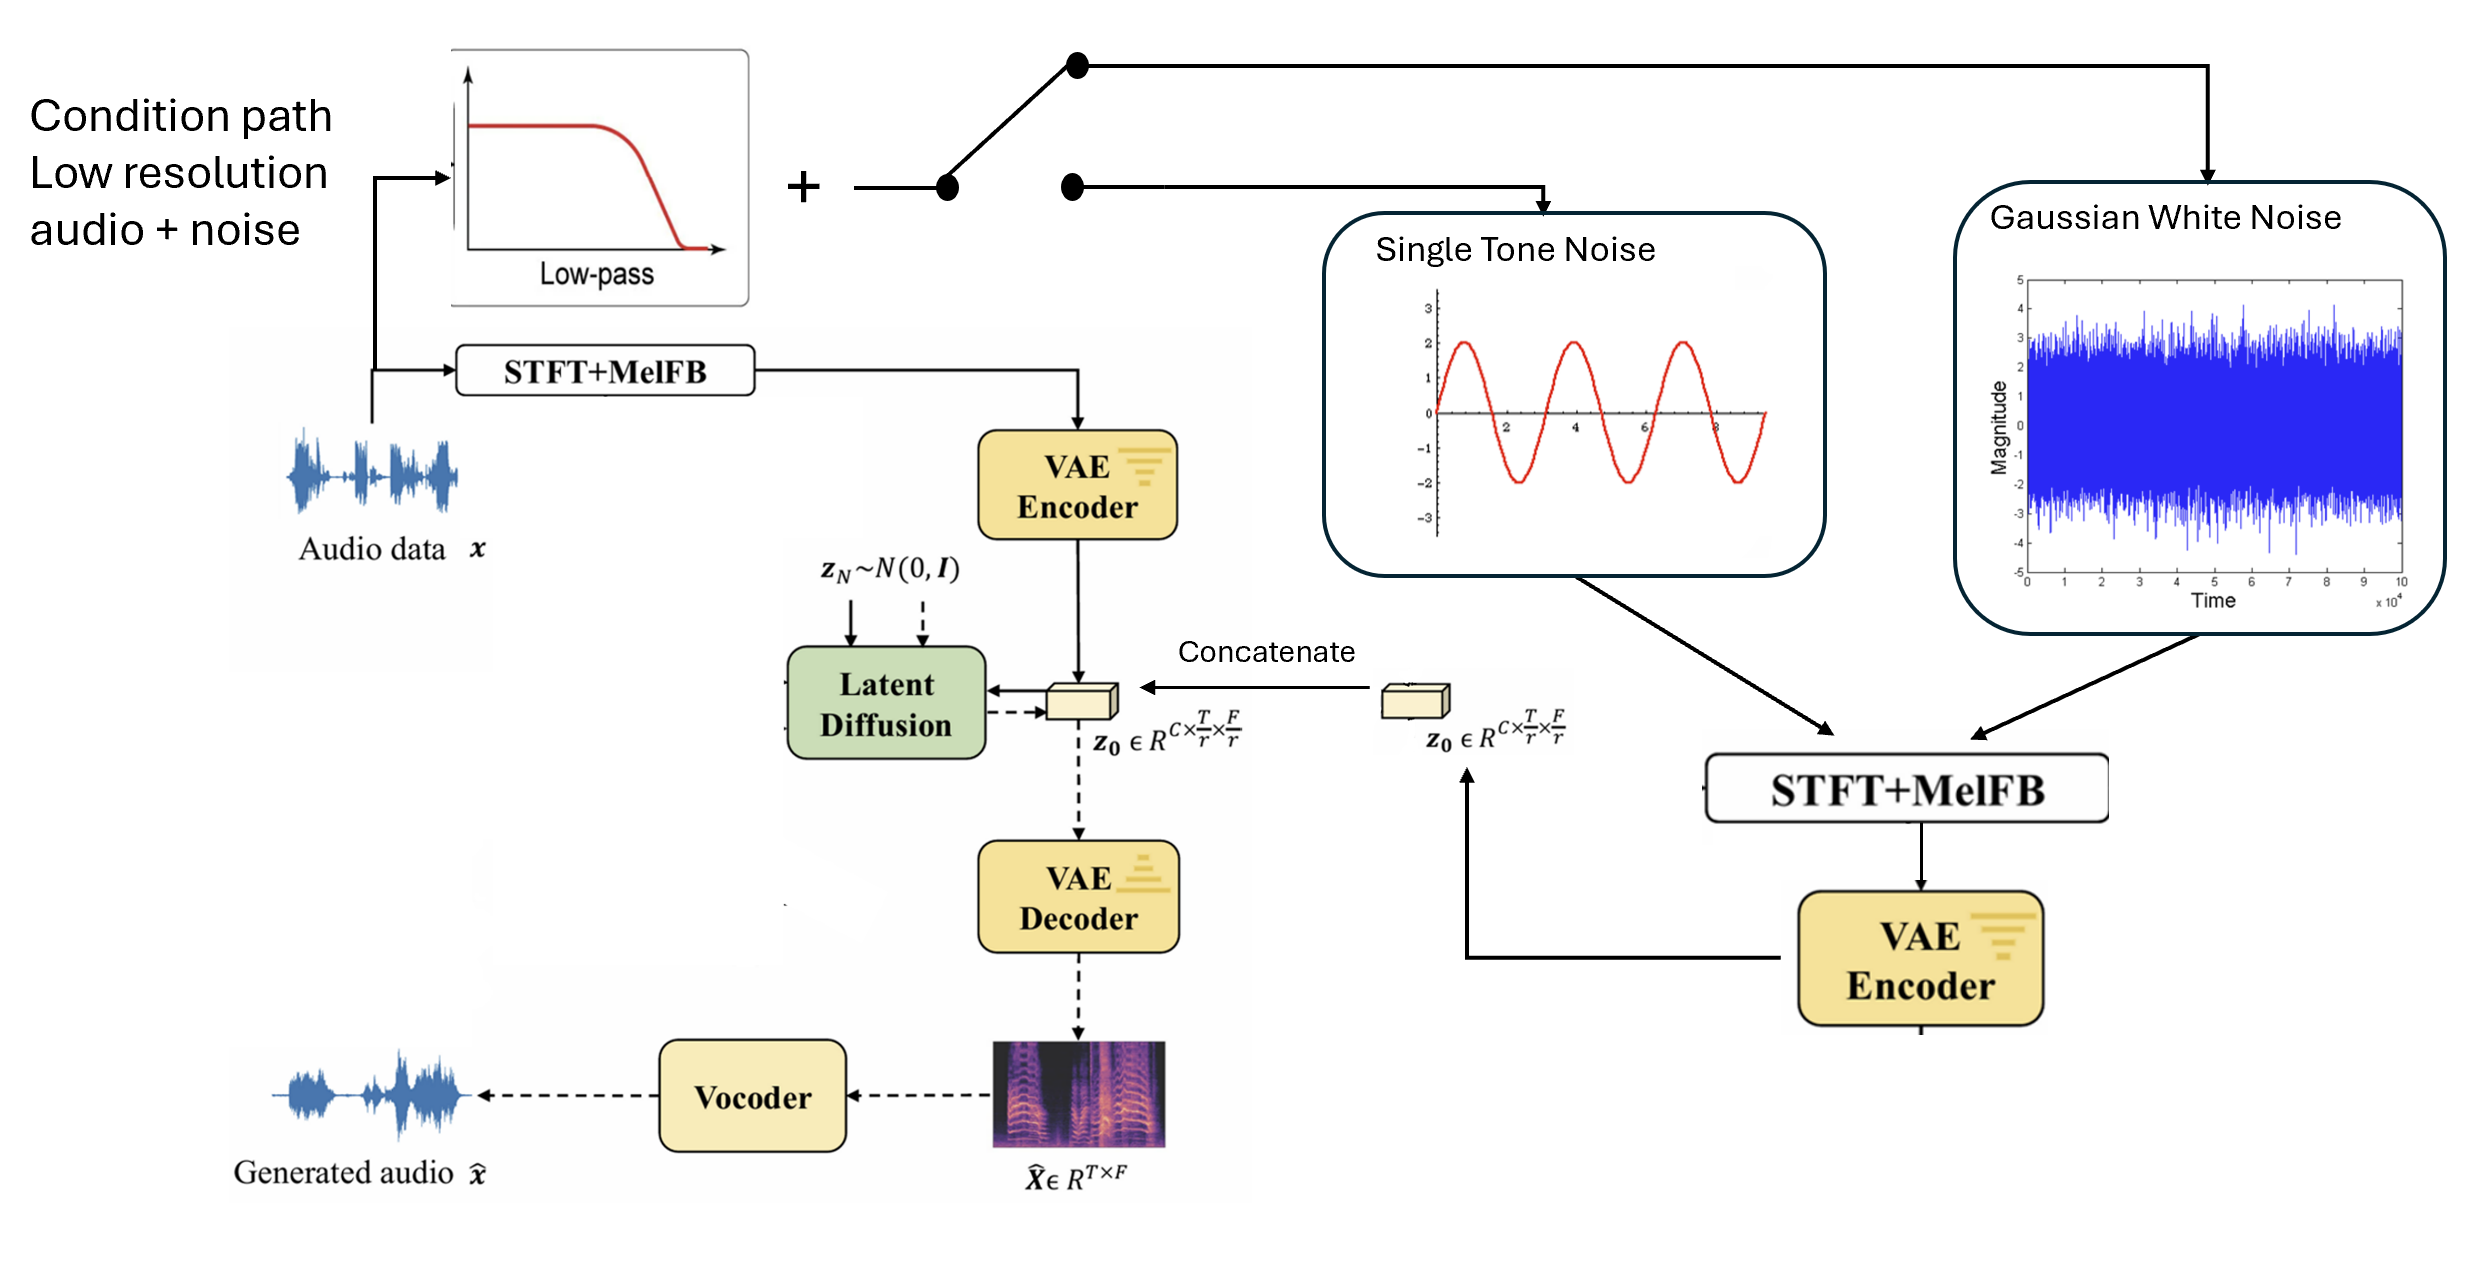
\includegraphics{images/audiosr_with_noise_architecture.png}
\caption{Architecture of AUDIOSR model plus noise}
\end{figure}

!!!!!!!!!!!! ADD HERE THE MATH AND EXPLANATION!!!!

\section{4. Preprocessing}\label{preprocessing}

In our study, we first apply a low-pass filter to the audio signal,
following the procedure outlined in AUDIOSR. The cutoff frequency for
the low-pass filter is randomly selected from a uniform distribution
between 2 kHz and 16 kHz. To ensure the robustness and generalization of
the filtering process, the type of low-pass filter is also chosen
randomly from four different filter designs: Chebyshev, Elliptic,
Butterworth, and Boxcar. The order of the filter is selected randomly
from an integer range between 2 and 10. This variability in the filter
selection is crucial to replicate the diverse conditions observed in the
referenced work and to address the filter generalization problem.

After filtering, we added noise to the waveform, randomly selecting
between single-tone noise and Gaussian white noise. For both types, the
amplitude is sampled from a uniform distribution. The amplitude range
for single-tone noise is set between 0.001 and 0.2, while for Gaussian
noise it is limited to 0.001 to 0.1, as Gaussian noise affects the
entire spectrum of the audio signal. The center frequency for the
single-tone noise is uniformly sampled between 100 Hz and 15 kHz.

\section{Data}\label{data}

The dataset used in this paper is MUSDB18 {[}??????{]}. MUSDB18 consists
of 150 full-length music tracks, totaling approximately 10 hours of
audio, with a dataset size of 4.4 GB. It is widely regarded as a
benchmark for music source separation tasks. The dataset includes a
collection of professionally produced songs spanning various genres,
such as rock, pop, jazz, and electronic music. Each track is provided as
a multitrack audio file, where the individual musical components are
separated into distinct ``stems,'' including vocals, drums, bass, and
other instruments. One of these stems contains the mixture of all
components, which we used for training purposes in this work.

\section{Experiment}\label{experiment}

In our experiment we divided the dataset as follow: 90 tracks were used
for the training, 10 for validation and 50 tracks for the test. We
followed the processes mentioned in the PROBLEM FORMULATION AND METHOD
section and in the PREPROESSING section to create the AUDIOSR
architecture using the AUDIOLDM architecture with the additional noise
components to the conditional part as demonstrated in Fig.????????

\section{Result}\label{result}

\section{Conclusion}\label{conclusion}

\section{Future Work}\label{future-work}

\section{References}\label{references}



\end{document}
